% Capítulo 1: símbolos básicos do fluxograma.
\documentclass[border=4pt]{standalone}
\usepackage[utf8]{inputenc}
\usepackage[T1]{fontenc}
% Estilo comum dos fluxogramas e diagramas de blocos.
\usepackage{tikz}
\usetikzlibrary{arrows.meta, positioning, calc, shapes.geometric, shapes.misc}
\definecolor{navy}{RGB}{23,45,80}
\definecolor{laranja}{RGB}{250,110,29}
\definecolor{cinzalogo}{RGB}{107,114,126}
\definecolor{azul}{RGB}{205,222,247}
\tikzset{
  base/.style={draw=navy, line width=0.9pt, font=\sffamily\small, align=center, inner sep=4pt},
  terminal/.style={base, rounded rectangle, fill=laranja!45, draw=laranja, minimum width=20mm, minimum height=7mm},
  processo/.style={base, rectangle, fill=laranja!12, minimum width=28mm, minimum height=8mm},
  decisao/.style={base, diamond, aspect=2.2, fill=azul, inner sep=1pt, minimum width=30mm},
  es/.style={base, trapezium, trapezium left angle=72, trapezium right angle=108,
             fill=white, minimum width=26mm, minimum height=8mm, trapezium stretches body},
  fluxo/.style={-{Stealth[length=2.2mm]}, navy, line width=0.9pt},
  rotulo/.style={font=\sffamily\small\bfseries, text=navy},
  legenda/.style={font=\sffamily\scriptsize, text=cinzalogo},
  resposta/.style={font=\sffamily\scriptsize\bfseries, text=navy},
}

\begin{document}
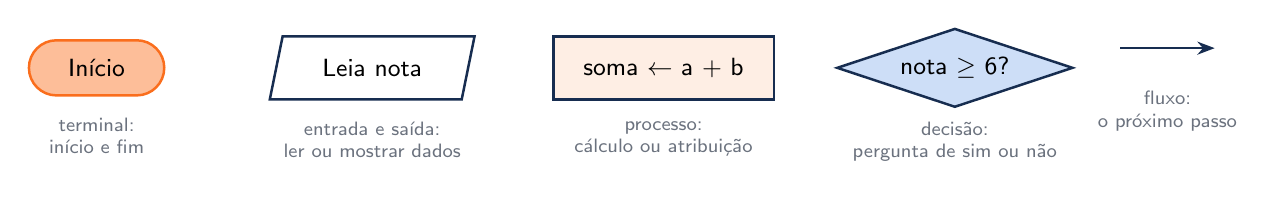
\begin{tikzpicture}
  \node[terminal] (t) at (0, 0) {Início};
  \node[legenda, below=1.5mm of t, align=center] {terminal:\\início e fim};

  \node[es] (e) at (3.5, 0) {Leia nota};
  \node[legenda, below=1.5mm of e, align=center] {entrada e saída:\\ler ou mostrar dados};

  \node[processo] (p) at (7.2, 0) {soma $\leftarrow$ a + b};
  \node[legenda, below=1.5mm of p, align=center] {processo:\\cálculo ou atribuição};

  \node[decisao] (d) at (10.9, 0) {nota $\geq$ 6?};
  \node[legenda, below=0.5mm of d, align=center] {decisão:\\pergunta de sim ou não};

  \draw[fluxo] (13.0, 0.25) -- (14.2, 0.25);
  \node[legenda, align=center] at (13.6, -0.55) {fluxo:\\o próximo passo};
\end{tikzpicture}
\end{document}
